\section{Data Availability}
\label{section:data-availability}

The Data Availability (DA) layer for L2 solutions outlines the method for storing 
information essential to recover L2 data in emergency situations.


\subsection{Synchronization on L1}
\label{section:data-availability:synchronization-on-l1}

To facilitate L2 data availability on the L1 network, the Synchronization Committee is introduced.
They ensure data availability on Ethereum for the entire 
zkSharding solution. 

Synchronization Committee participants hold a distinct role in zkSharding. 
The committee is formed by validators who opt for this additional role.
The committee operates in epochs defined by the protocol parameters,
 with a new committee elected each epoch.
An account cannot be an active validator 
 and a member of the Synchronization Committee simultaneously; 
 this separation is enforced by the committee election algorithm.
Therefore, although committee members use the same stake, 
 these funds are eligible for slashing for only one role at any given time.

Following a period of time defined by the protocol parameters, 
 the committee generates a state difference for the shard between time T and T + p.
The protocol is operated via application on top of the \mainshard.
A selected node proposes the hash of the state difference and the Synchronization Committee votes on it. 
Upon achieving $\frac{2}{3} + 1$ votes, the state difference, its hash, and the aggregated signature 
 are composed into an Ethereum data availability transaction. 
In case of achieving $\frac{1}{3}$ votes "against" the proposed difference, the leader is slashed.

If multiple Ethereum transactions are prepared, the committee may 
decide to compose them into an L1 block. This enables participation in Relayer auctions and 
achieves soft finality faster by including the block in the nearest current epoch slot (Figure \ref{figure:soft-finality}). 
Alternatively, in case of too few Ethereum DA or state-proof transactions, they can be sent 
directly to the builders/searchers (as bundle or transaction).

\begin{figure}[h]
    \centering
	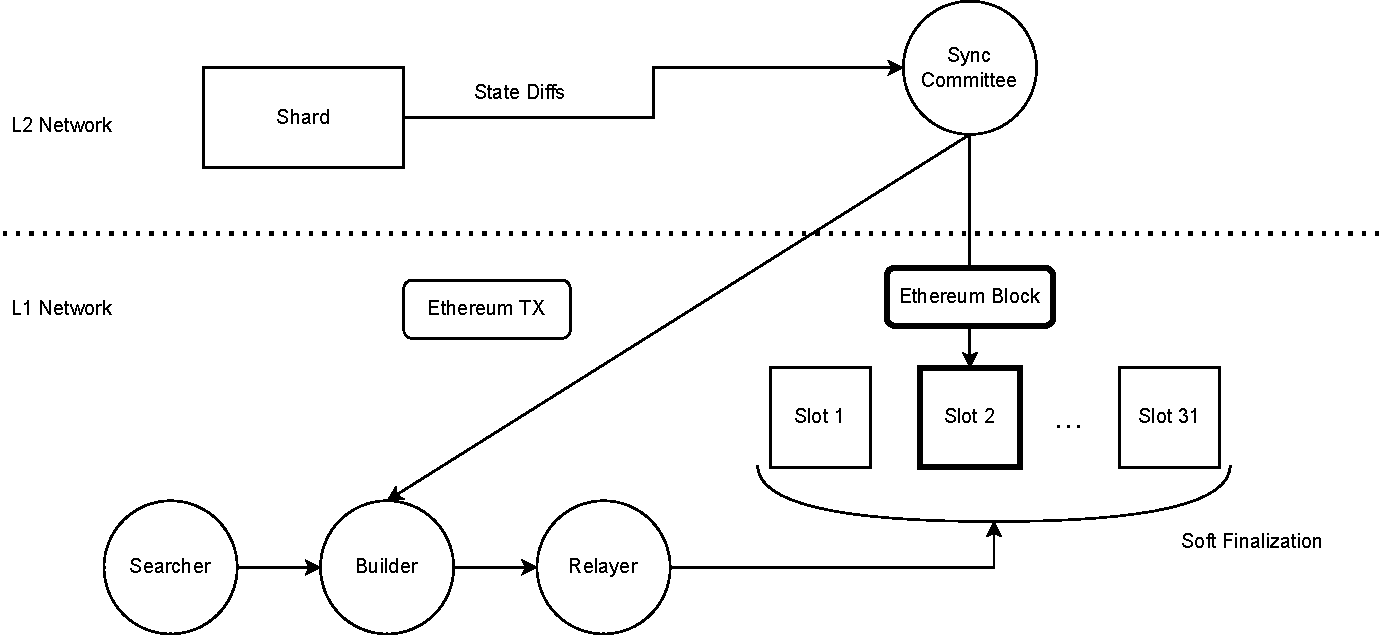
\includegraphics[scale=0.65]{figures/soft-finalization.pdf}
    \caption{Synchronization on L1}
     \label{figure:soft-finality}
\end{figure}


\subsection{\mainshard}

The \mainshard periodically submits its snapshot to Layer 1 (L1) in the form of the state 
differentials. These state differentials represent the modified segments of the global state 
resulting from the application of L2 transactions to the previous state. The purpose of these 
differentials is to aid in reconstructing a complete L2 state by integrating sequential historical 
changes in case of rollback events.

Given that the \mainshard is responsible for storing and synchronizing the latest state roots 
committed by execution shards, the transactions it handles are highly specific and persistent 
in their computations and storage usage.


\subsubsection{Finalization}

Probabilistic (soft) finalization is attainable due to the high reliability of Ethereum validators. 
The achievement of probabilistic finalization happens when the \mainshard's data availability 
transaction is verified in the L1 slot.

On the other hand, hard finalization is only accomplished after the verification process. 
The state change proof, coupled with fully finalized state differences, is necessary for the 
finalization of Layer 2 defined as follows:

\[
    Finalization_t =
    \left\{
    \begin{array}{lr}
    true, & \text{if } V_{zk}(proof_t) \wedge V_{diff}(Diff_t), where: V - verification function\\
    false, & \text{otherwise}
    \end{array}
    \right\}
\]
    

\subsubsection{Data organization and store}

Data on L1 is stored in a specifically deployed contract, tasked with accepting L2 state differences, 
verifying signatures, and persistently storing the data on the chain. Each submitted L2 \mainshard 
state difference is stored in Ethereum $calldata$ while metadata on storage as a sequential chain, and 
the structure appears as mapping:

\begin{verbatim}
    head: hash32;
    mapping (hash32 => struct) {
        signature : hash32,
        da_hash : hash32, 
        period : uint32 (>= 1),
        prev_da : hash32,
        zk_proof_hash : hash32,
        zk_verification_passed : bool
    }
\end{verbatim}


State transition proof and state differential hashes will serve as the means for navigating the data stored 
in $calldata$. 
The verification status can only be set after the successful validation of the state 
transition proof. 
The term "period" refers to the number of blocks that are consolidated. Since this 
number is not fixed and is defined by the protocol parameters, it must be explicitly stored.

\subsubsection{Transactions cost impact}

The primary content in the data availability transaction submitted to L1 consists of the state 
roots submissions from execution shards to the \mainshard. 
As mentioned earlier, the influence 
of transactions on \mainshard storage remains relatively constrained. 
Although the fundamental 
idea of sharding revolves around limitless horizontal scaling, the calculations are presently 
centered on achieving the current target of 60,000 transactions per second (TPS) with 400 execution shards. 

Execution shards submit relatively lightweight transactions to the \mainshard, primarily focused 
on submitting the latest state root after each new block. 
Simultaneously, the \mainshard is expected 
to submit data availability during intervals measured in blocks an interval adjustable by the protocol parameters. 
GPT
For the calculations, a value equal to half of the Ethereum slot time, which is 6 seconds, was chosen.
The system produces one block per second.

Every execution shard transaction will result in a change to its account nonce value (32 bytes), 
balance ($32$ bytes), and storage ($32$ bytes state root hash). 
It's worth noting that the Merkle State 
Trie path, in this case, is considered to have an average depth of 3. 
The probability of choosing two 
identical 3-byte prefixes for $400$ keys is approximately $0.475$\%, which can be safely accepted as 
the worst case.

\[
\texttt{size} = \texttt{shards} \cdot (\texttt{nonce} + \texttt{storage} + \texttt{balance} + \texttt{merkle\_path}) = 400 \cdot 32 \cdot 6 = 76800 \texttt{ bytes}
\]


The total data size, excluding metadata, is $76.8$ kilobytes. The metadata and aggregated committee 
signatures are relatively small and can be disregarded.

Given the high entropy nature of the data, the ratio of zeros to non-zeros in the data packet is 
approximately $\frac{1}{256}$. This results in:

\[
    Gas_{zero} = \frac{1}{256} \cdot 76800 \cdot 4(\texttt{gas\_cost}) = 1200
\]
\[
    Gas_{non-zero} = \frac{255}{256} \cdot 76800 \cdot 16(\texttt{gas\_cost}) = 1224000
\]
\[
    Gas_{total} = Gas_{zero} + Gas_{non-zero} = 1225200
\]


At the current ETH cost of \$2900 and a gas price of $15$ gwei, the approximate cost of the Data 
Availability transaction is \$53.2962.

It is important to note that this calculation does not account for the diffs period. The rationale 
behind this omission is that the commitments size of the diffs remains consistent, given that the 
changes involve the same accounts.

It is important to note that this calculation does not account for the state diffs period. 
The rationale behind this omission is that the commitment size of the diffs remains consistent, 
given that the changes involve the same accounts.

However, the estimated additional cost fee for L2 transactions related to DA can be calculated as 
$1225200 / (6 \cdot 60000) = 3.403$ gas or \$0.00014 per user transaction. In comparison, it will be 6 
times higher (\$0.00084) in the case of submission each main submission. It's crucial to acknowledge 
that increasing the period for state diffs may compromise stability, particularly in the event of a 
\mainshard revert where the entire state diff period must be reverted across all shards.


\subsection{Execution Shards}

The paper does not outline specific requirements for data availability in the execution shards. 
Nevertheless, it is recommended to bolster the shard's security by storing snapshots on a reliable 
off-chain solution. For instance, each execution shard can autonomously merge state differences over 
a designated period, compress the data, and then submit it to the Ethereum network (as "calldata" or 
by EIP-4844) or a dedicated Data Availability layer solution.

\subsubsection{Continuous state difference merge (CSDM)}


EIP-4844 introduces substantial improvements for all L2 solutions on the Ethereum network. 
To harness the full capabilities of this new standard and unlock significant cost reduction potential for zkSharding, 
 the CSDM mechanism is introduced to enhance data availability for execution shards.

In alignment with the Ethereum philosophy of verification, this data availability mechanism 
also incorporates complete persistence of the shard's state on temporary storage. 
% The high-level 
% concept is illustrated in Figure 3.
% \todo{insert image from Petr and rename figure}

The process is divided into three parts: initialization, state difference saving, and merge. 
During the initialization stage, execution shards store the full state in a blob at time $T$ for 
a duration of n periods. Subsequently, at regular intervals of time $p$ (blocks), the execution 
shard saves the state difference, $D$, between $T+pk$ and $T+p(k+1)$. The merge operation takes place 
at time $T+n$ when the shard executes the following operation:

\[
    S_{T+n} = \hat{Y}(...(\hat{Y}(\hat{Y}(S_T, D_{T+p}), D_{T+2*p})..., D_{T+n}),
\]
where $\hat{Y}$ is the state merge function defined as $S_{T+k} = \hat{Y}(S_T, D_{T+k})$.

The rationale behind the mechanism can be substantiated by examining the evidence of saving 
state differences during the time. Suppose there is a throughput of 60,000 TPS, 256 million 
unique accounts (statistics from Ethereum), 1 second block generation time (1 BPS, blocks per second).

Given the BPS and TPS figures,
 it is asserted that the minimum number of changed accounts will be at least 60,000, 
 since only externally owned accounts (EOA) can create transactions.

In each new block, the distribution of unique accounts (transactions) follows a normal 
(Gaussian) distribution as a natural process. If updates occur every 90 days, the total 
number of changes will be $seconds * TPS = 466560000000$. Utilizing a generally calculated 
standard deviation, the probability of changing all 256 million accounts is very high (94.51\%), 
and the probability of changing 90\% is even higher (99.93\%). This renders it entirely 
reasonable to fully update and resave the state, as the changes during this time effectively 
create an entirely new state.